% !TeX root = ../thuthesis-example.tex

\chapter{Introduction}
\label{chap:1}

Enzymes are proteins that catalyze biological reactions. They accelerate reactions 
to a speed that supports metabolic processes necessary for life. 
Understanding how enzymes work is crucial not only for understanding fundamental 
biological mechanisms but also for advancing medical science, 
particularly in the development of new pharmaceuticals and the engineering 
of enzymes with enhanced properties.

In order to design effective drugs or improve enzyme functions, 
one major challenge is the selection of the most promising compounds 
from a vast array of possibilities. 
Laboratory testing is costly and time-consuming. To reduce the possibilities,
using kinetic information can become a promising solution.

A key parameter in enzyme kinetics is the Michaelis constant ($K_m$). It represents
the substrate concentration at which the initial velocity of the reaction is half of
the maximum velocity. Generally, the lower the value, the higher is the affinity 
between the enzyme and the substrate.

Therefore, predicting the Michaelis constant can significantly accelerate the drug design process. 
By estimating an enzyme's affinity for various substrates and similarly, several enzymes
with one substrate, researchers can prioritize compounds for further development, 
thereby reducing the need for extensive laboratory testing. 
This approach not only facilitates the discovery of new drugs but also enhances 
our ability to engineer enzymes with desired characteristics.

\section{Problem statement}

The goal of this work is to build a statistical regression model that predict the 
Michaelis constant given 2 inputs: the protein sequence and the substrate string. 

The performance of the model will be evaluated with the mean squared error (MSE) and 
the coefficient of determination $r^2$, following current evaluation techniques for this task.

\section{Literature review}

Given the interdisciplinary nature of this thesis, which involves biological, chemical, and 
computer sciences, the literature review will be structured in the following way.

First, we introduce the biological and chemical fundamentals necessary to understand basic aspects
of enzyme kinetics. This foundation is essential to comprehend the biological processes at play and
their relevance to our work.

Second, machine learning and deep learning methodologies, emphasizing on their biological
applications, will be presented. This section aims to present how statistical models can be used to decipher complex biological
data, hence allowing us to build innovative solutions in enzyme and drug design.

Finally, we delve into the current state of research regarding the prediction of the Michaelis 
constant ($K_m$). The aim of this part is to highlight the current contributions to 
our problem statement, the current state-of-the-art methods used, and their results.

Through this comprehensive review,the solid background provided will ensure the relevance of this thesis
contribution in the field of drug design.

\subsection{Biological and Chemistry Background}
\subsubsection{Proteins}
Proteins impact all the processes that take place in a cell, with an almost
endless diversity of functions. They are the most abundant biological macromolecules.
Thousands of different types of proteins can be found in a single cell. They are the molecular
instruments through which genetic information is expressed.\cite{lehninger}

A protein is a sequence of smaller molecules called amino acids that are covalently joined by a peptide
bond. There exists 20 common amino acids (Figure \ref{fig:20aa}) from which almost all proteins are made of. Each amino acid has
a side chain with distinctive chemical properties.

\begin{figure}
  \centering
  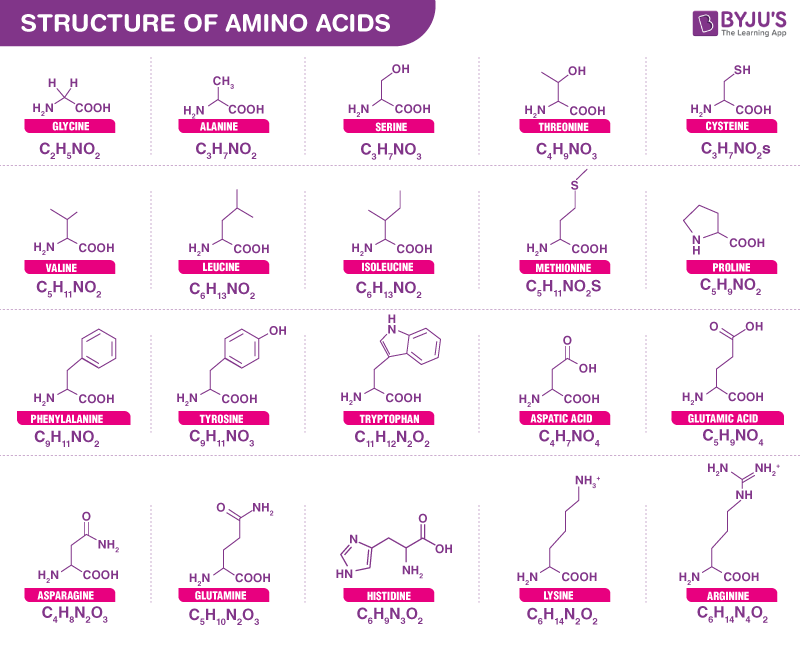
\includegraphics[width=0.7\linewidth]{1-amino_acids.png}
  \caption{The 20 common amino acids. Adapted from \citeauthor{BYJUsAminoAcids}.}
  \label{fig:20aa}
\end{figure}

All common amino acids are $\alpha$-amino acids. This means that both the carboxyl group and the amino group
is bonded to the same carbon atom called the $\alpha$-carbon (Figure \ref{fig:aastructure}). The amino acids differ from each others in
their side chains, also called R-groups, which vary in size, structure, electronic charge, and which
influence the solubility of the amino acids in water.

\begin{figure}
  \centering
  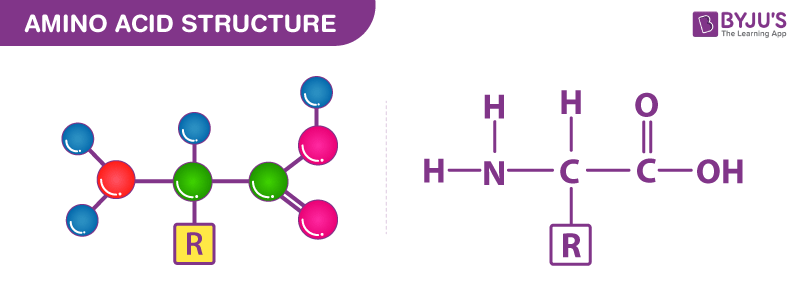
\includegraphics[width=0.7\linewidth]{1-amino_acid_structure.png}
  \caption{Amino acid structure. Adapted from \citeauthor{BYJUsAminoAcidsStructure}.}
  \label{fig:aastructure}
\end{figure}

Two amino acids can be joined together with a covalent bond that is called a peptide bond. This link
is formed by the removal of the element of water (a hydroxyl group from the $\alpha$-carboxyl group
of one amino acid and a hydrogen atom from the $\alpha$-amino group of another amino acid. Figure 
\ref{fig:peptidebond}). These joined amino acids are called residues, relfecting the loss of the element
of water during the bonding formation.

\begin{figure}
  \centering
  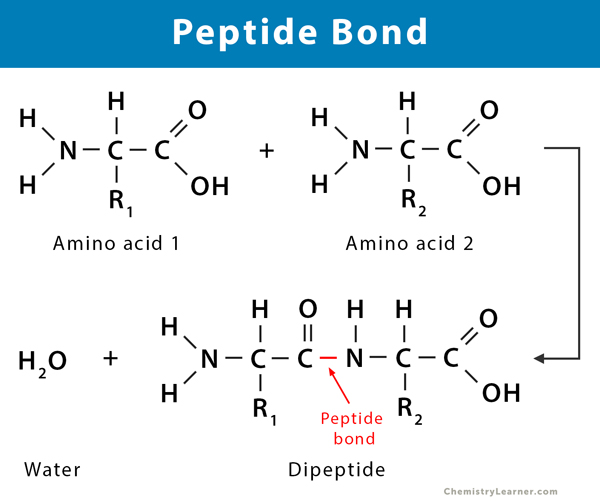
\includegraphics[width=0.7\linewidth]{1-peptide_bond.jpeg}
  \caption{Peptide bond. Adapted from \citeauthor{ChemistryLearnerPeptideBond}.}
  \label{fig:peptidebond}
\end{figure}

An oligopeptide is the structure of a few amino acids joined together and a polypeptide is the name
given to the structure when many amino acids are joined. Proteins may have thousands of amino acids residues.

For proteins, the amino acid residues at the end are the $\alpha$-amino group called N-terminal and 
the $\alpha$-carboxyl group called C-terminal. The N-terminal is conventionally placed on the left while
the C-terminal is placed on the right.

The functions of proteins do not depend on their length or molecular weight. \cite{Alberts2002ProteinFunction} Some very small proteins 
(2 to 10 amino acids) can be extremely important such as insuline, a hormone crucial for regulating blood sugar levels. 
Although human insulin consists of 51 amino acids (making it relatively light and small compared to many other proteins), 
it plays a vital role in metabolism. \cite{Steiner1985} The length of proteins can vary enourmously 
from 2 to 27,000 amino acids, while the vast majority of proteins usually contain fewer than 2,000 amino acids.

Some proteins are made of only one polypeptide chain while other can be made out of several, they are 
called mutlisubunit proteins, such as hemoglobin which is composed of four polypetide chains (two alpha
and two beta chains) and iron-containing heme groups. \cite{Perutz1970} 
It is essential for oxygen transport in the blood.

\begin{figure}
  \centering
  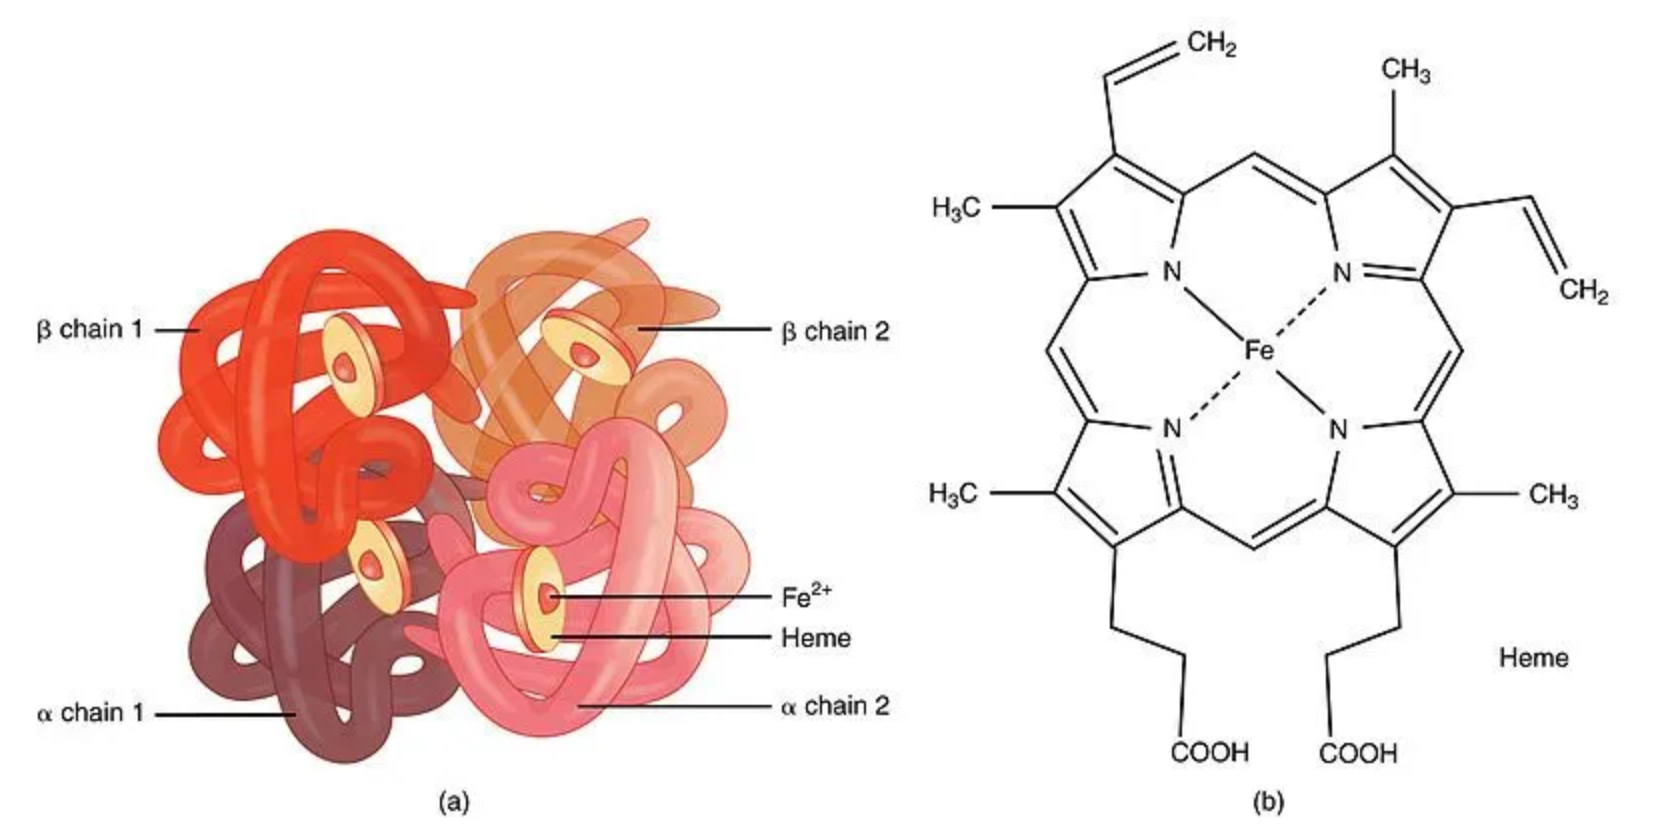
\includegraphics[width=0.7\linewidth]{1-hemoglobin.png}
  \caption{(a) Hemoglobin molecule. (b) Heme iron. Adapted from \citeauthor{ALevelBiologyHemoglobin}.}
  \label{fig:hemoglobin}
\end{figure}

Some proteins also contain chemical groups other than amino acids. They are called conjugated proteins.
The non-amino acid part of these proteins is called its prosthetic group and is essential to the protein
overall functions. Chlorophyll, a protein essential for photosynthesis by allowing plants to absorb energy
from light is a perfect example. \cite{Photosynthesis}

The vast diversity in protein structure, from simple monomeric forms to complex multisubunit 
configurations, underlines their ability to perform a wide array of biological functions. 
Beyond structural roles and hormone regulation, proteins are pivotal in catalyzing biochemical 
reactions, a role exemplified by enzymes. Enzymes, a specialized class of proteins, are a perfect example of the 
functional versatility of proteins. 

\subsubsection{Enzymes}
\label{section:enzyme}
Enzymes are specific proteins that accelerate the rate of reactions. They are essential to life as many
of the chemical reactions essential to our survival need to be accelerated, such as lipases that are 
a group of proteins that helps digest fats in the gut. \cite{Pirahanchi2023Lipase} 
They are also essential to regulate the vast network of metabolic pathways necessary for life. An example
of this is the enzyme phosphofructokinase (PFK) which regulates glycolisis, the production of glucose
based on the cell requirements. \cite{Kanai2019Phosphofructokinase}

With the exception of a few classes of catalytic RNA molecules, enzymes are proteins. 
Their catalytic activity depends on the integrity of their native protein conformation. 

If an enzyme is denatured or dissociated into its subunits, catalytic activity is usually lost. 
The catalytic activity of each enzyme is deeply linked to its primary, secondary, tertiary, 
and quaternary protein structure.

Some enzymes require a chemical component called cofactor - either one or more inorganic ions 
such as Fe2+, Mg2+, Mn2+ or Zn2+, or a complex organic or metalloorganic molecule called coenzyme. 
Coenzymes act as transient carriers of specific functional groups. Most are derived from vitamins.
Some enzymes require both a coenzyme and one or more metal ions for activity. A coenzyme or metal ion 
that is very tightly or even covalently bound to the enzyme protein is called a prosthetic group. 
A complete catalytically active enzyme with its bound coenzyme/or metal ion(s) is called a holoenzyme. 
The protein part of such an enzyme is called the apoenzyme or apoprotein.

While many enzymes have the suffix "-ase" to the name of their substrate or to a word describing
their activity, there exists a convention system to classify all enzymes, it is called the Enzyme Commission
(EC) system. \cite{EC} It divides enzymes into 7 classes, each with subclasses, based on the type of reaction
catalyzed. Each enzyme is assigned a 4-part classification number and a systematic name, which
identify the reaction it catalyzes.

\begin{table}[h!]
  \centering
  \begin{tabular}{ll}
  \hline
  \textbf{Number} & \textbf{Name} \\
  \hline
  1 & Oxidoreductases \\
  \hline
  2 & Transferases \\
  \hline
  3 & Hydrolases \\
  \hline
  4 & Lyases \\
  \hline
  5 & Isomerases \\
  \hline
  6 & Ligases \\
  \hline
  7 & Translocases \\
  \hline
  \end{tabular}
  \caption{Enzyme Commission Number and Names}
  \label{table:enzyme_names}
  \end{table}  

Under biologically relevant conditions, uncatalyzed reactions tend to be slow as most biological molecules
are quite stable in the neutral-pH, mild-temperature, aqueous environment inside cells.

What is special about enzyme-catalyzed reaction is that they take place in a pocket on the enzyme
which is called the active site. It provides a specific environment, customized by evolution, in which
a given reaction can occur more rapidly. 
The molecule that is bound in the active site and acted upon by the enzyme is called the substrate.
The surface of the active side is made of amino acid residues with R-groups that can bind the 
substrate and catalyze its chemical transformation. The substrate is often enclosed by the active site, 
sequestered completely from the solution.
The enzyme-substrate complex is central to the action of enzymes and is also the basis for kinetics models.

An enzymatic reaction can be describe as $E+S=ES=EP=E+P$ where $E$, $S$, and $P$ represent the enzyme,
substrate, and product respectively. $ES$ and $EP$ are transient complexes of the enzyme with the substrate
and with the product. The function of a catalyst is to increase the rate of reaction. It does not affect
reaction equilibria. 

In the coordinate diagram, the free energy of the system is plotted against the progress of the reaction. 
The starting point for either the forward reaction or the reverse reaction is called the ground state.

\begin{figure}
  \centering
  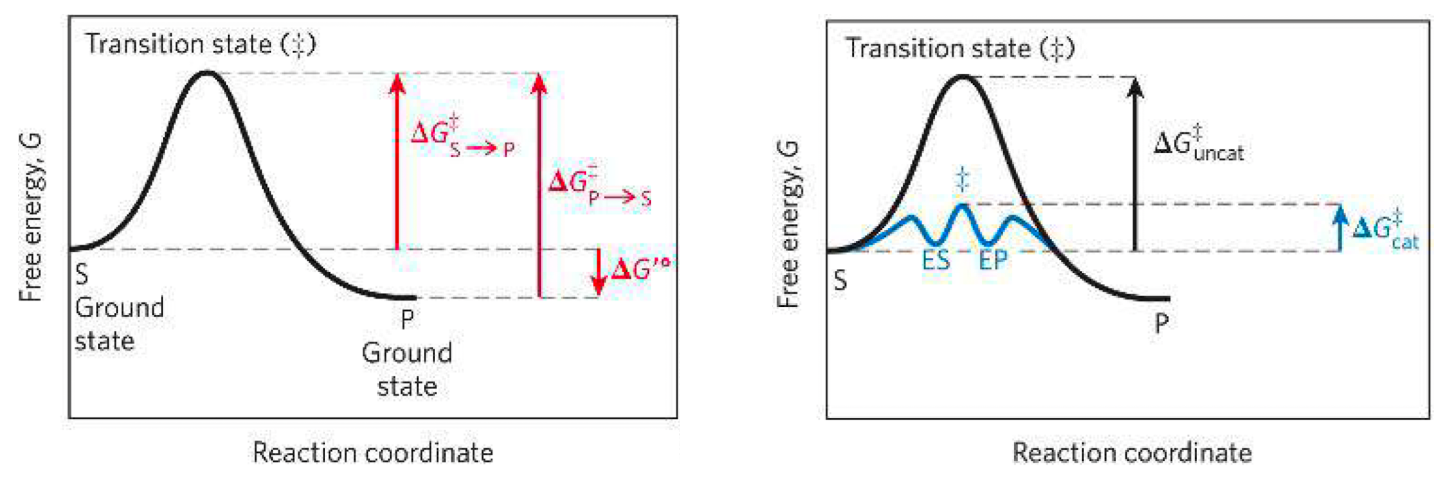
\includegraphics[width=0.7\linewidth]{1-coordinate_diagram.png}
  \caption{On the left, the coordinate diagram of an uncatalized reaction. On the right, the coordinate diagram of a enzyme-catalyzed reaction. Adapted from \citeauthor{lehninger}}
  \label{fig:coordinate_diagram}
\end{figure}

As a convention, we express the standard free-energy change $\Delta G˚$ at 298K, 
1atm for each gas, and concentration of each solute 1M.

Because biochemical systems commonly involve H+ concentration far below 1M, we define 
a biochemical standard free-energy change $\Delta G'˚$, the standard free-energy 
change at pH 7.

The equilibrium between S and P reflects the difference in the free energies of their ground states. 
Here, the free energy of the ground state P is lower than that of S so $\Delta G'˚$ is 
negative (exergonic reaction) and at equilibrium there is more P than S.

A favorable equilibrium does not mean that the S→P conversion will occur rapidly. The rate of a 
reaction depends on a completely different parameter: the energy barrier between S and P. It consists 
of the energy required for the alignment of reacting groups, formation of transient unstable charges, 
bond rearrangements, and other transformations required for the reaction to proceed in either direction.

To undergo reaction, the molecules must overcome this barrier and therefore be raised to a higher 
energy level. At the top of the energy hill is a point at which decay to the S or P state is 
equally probable (downhill either way). This is called the transition state ($\ddag$).

The transition state is not a chemical species with any significant stability and should not be 
confused with a reaction intermediate such as ES or EP. It is simply a fleeting molecular moment 
in which events such as bond breakage, bond formation, and charge development have proceeded to the 
precise point at which decay to substrate and decay to product are equally likely. 

The difference between the energy level of the ground state and the energy level of the 
transition state is the activation energy $\Delta G^\ddag$. The rate of a reaction reflects 
this activation energy: a higher activation energy corresponds to a slower reaction. Hence 
lowering the activation energy increases the rate of reaction. 

This can be done by raising the temperature or pressure, thereby increasing the number 
of molecules with sufficient energy to overcome the energy barrier. It can also be done by adding a 
catalyst that lower the activation energy, which is what enzymes do. 
Catalysts do not affect reaction equilibria. The role of enzymes is to accelerate the 
interconversion of S and P. 

Any reaction may have several steps, involving the formation and decay of transient chemical 
species called reaction intermediates.
A reaction intermediate is any species on the reaction pathway that has a 
finite chemical lifetime (longer than a molecular vibration ~$10^{-13}$ second). When 
the $S=P$ reaction is catalyzed by an enzyme, the $ES$ and $EP$ complexes can be considered intermediates, 
even though S and P are stable chemical species. 
Additionally, less-stable chemical intermediates often exist in the course of an enzyme-catalyzed 
reaction. The interconversion of 2 sequential reaction intermediates thus constitutes a reaction step.
When several steps occur in a reaction, the overall rate is determined by the step(s) with 
the highest activation energy; this is called the rate-limiting step. 
It is the highest-energy point in the diagram for the interconversion of S and P. It can vary 
with reaction conditions, and for many enzymes several steps may have similar activation energies, 
which means they are all partially rate-limiting.

Activation energies are energy barriers to chemical reactions. They are crucial to life 
itself. Without such energy barriers, complex macromolecules would revert spontaneously 
to much simpler molecular form, and the complex and highly ordered structures and metabolic 
processes of cells could not exist.


\subsubsection{Pocket detection}
xxxx

\subsubsection{Enzyme Kinetics}
At all time in an enzyme-catalyzed reaction, the enzyme exists in 2 forms: the free and uncombined 
form $E$ and the substrate-combined form $ES$.
When the enzyme is first mixed with with a large excess of substrate, there is an initial 
transient period, the pre-steady state, where the concentration of $ES$ accumulates.
For most enzymatic reactions, this period is very brief, frequently too short to be observed easily, 
lasting only the time required to convert one molecule of substrate to product.
The reaction then achieves a steady state, in which $[ES]$ remains approximately constant for much of 
the remainder of the reaction. As most of the reaction reflects the steady state, the traditional 
analysis of reaction rates is referred to as steady-state kinetics.

A key factor affecting the rate of a reaction catalyzed by an enzyme is the concentration 
of substrate, $[S]$.
It is hard to study the effects of substrate concentration because $[S]$ changes 
during the course of an in vitro reaction as substrate is converted to product. 
One approach is to measure the initial rate, $V_0$.

At the beginning of the reaction, we can consider the concentration of $[S]$ constant and
 $V_0$ increases almost linearly with an increase in $[S]$. 
At higher substance concentrations, $V_0$ increases by smaller and smaller amounts, in response 
to an increase in $[S]$. Finally, a point is reached beyond which increases in $V_0$ are 
vanishingly small as $[S]$ increases. This plateau-like $V_0$ region is close to the 
maximum velocity, $V_{max}$.

\begin{figure}
  \centering
  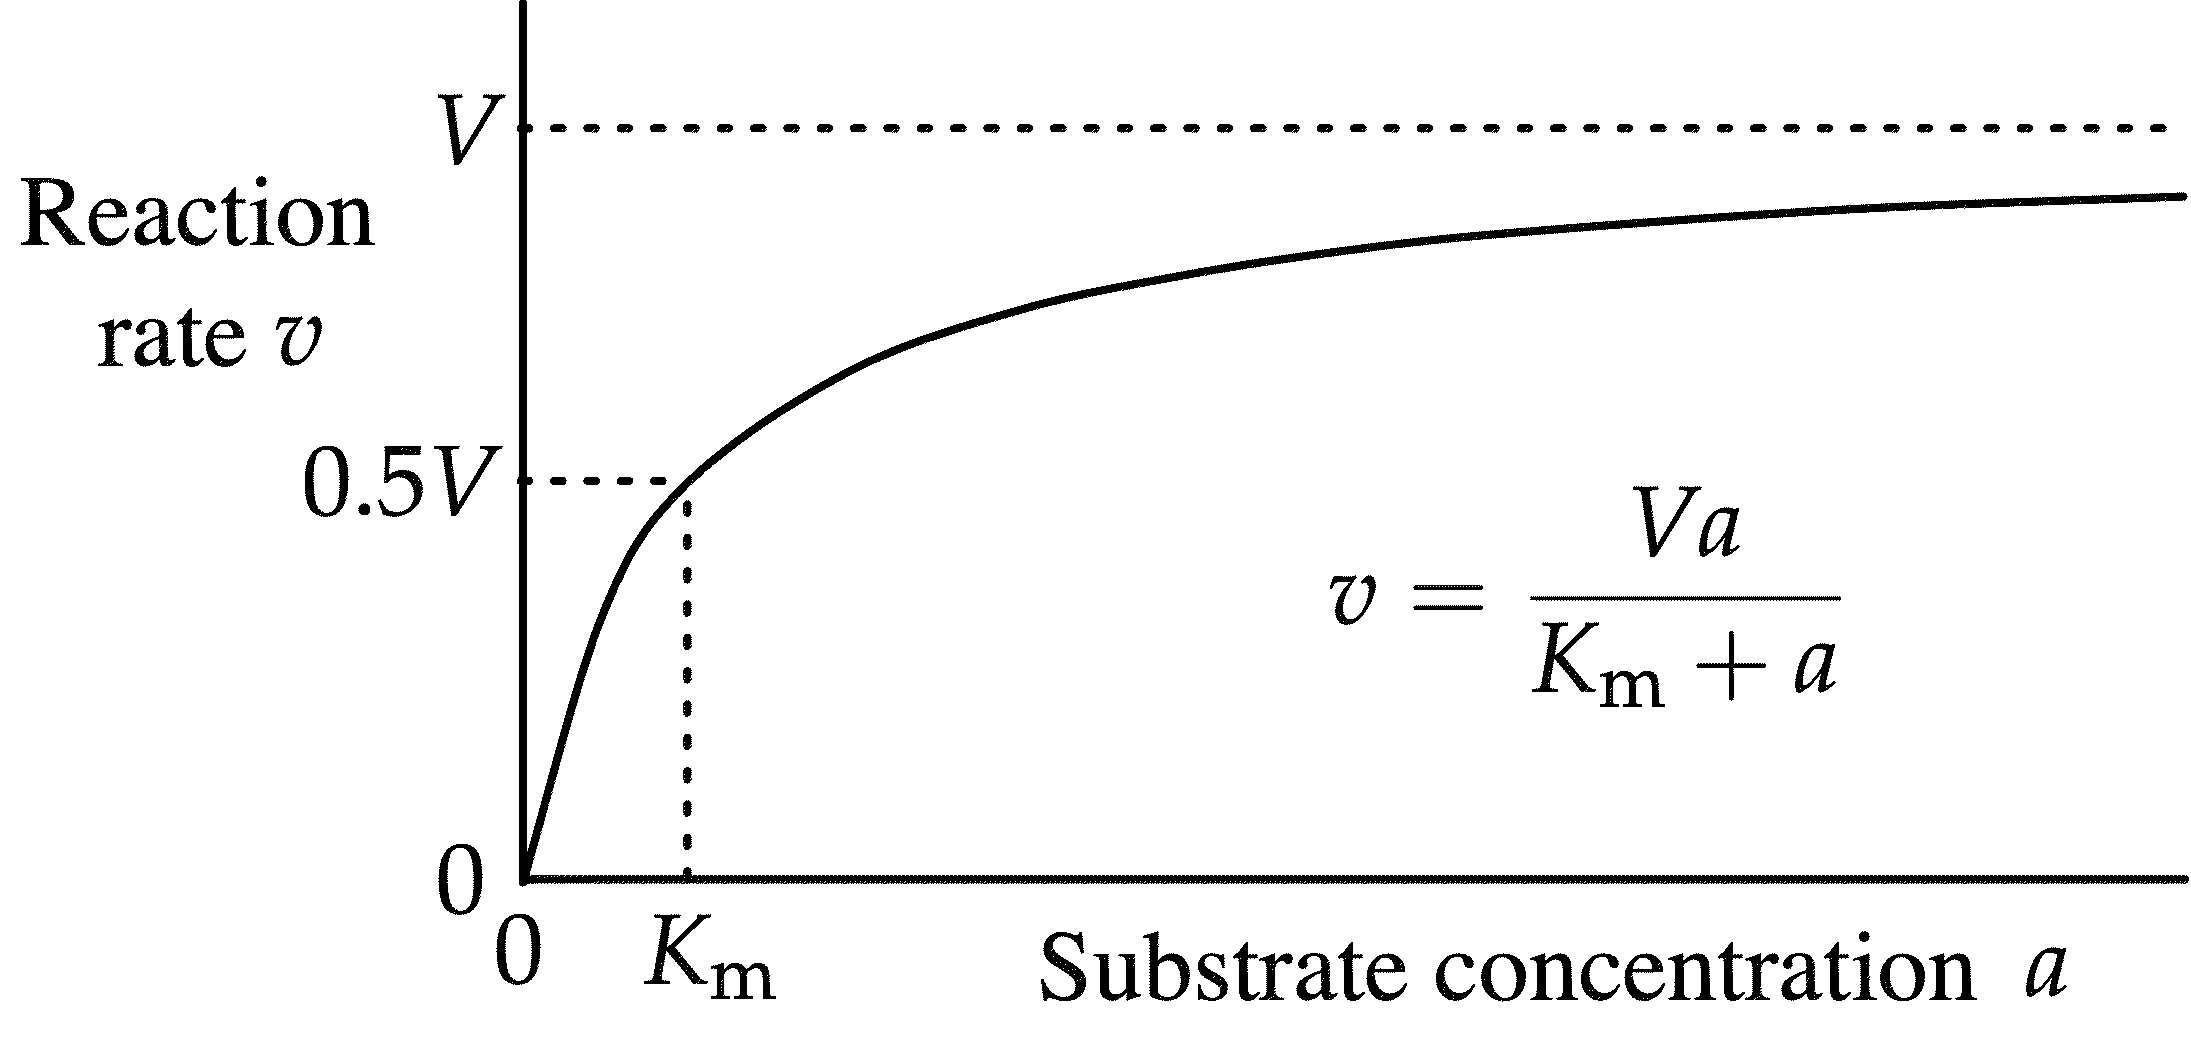
\includegraphics[width=0.7\linewidth]{1-mm_curve.jpeg}
  \caption{Michaelis-Menten kinetics. Adapted from \citeauthor{lehninger}}
  \label{fig:mm_curve}
\end{figure}

The ES complex is key to understanding this kinetic behavior. There are two equations: $E+S=ES$ 
and $ES(=EP)=E+P$ with the formation of the complex and then formation of the product.
The second reaction is slower and limits the rate of the overall reaction. 
Then, the overall rate must be proportional to the concentration of the species that reacts in 
the second step, that is $ES$.

At low $[S]$, most of the enzyme is in the uncombined form $E$.
The maximum initial rate of the catalyzed reaction Vmax is observed when virtually all the enzyme 
is present as the ES complex and $[E]$ is very small.
Under these conditions, the enzyme is “saturated” with its substrate, so that further increases 
in $[S]$ has no effect on the rate. $[S]$ needs to besufficiently high so that the enzyme is 
mostly in the $ES$ form.
After the $ES$ complex breaks down to yield the product $P$, the enzyme is free to catalyze the reaction 
of another molecule of substrate (and will do so rapidly under saturating conditions). The saturation 
effect is a distinguishing characteristic of enzymatic catalysts and is responsible for the plateau 
of $V_0$.

\paragraph{Michaelis-Menten equation}

The curve of the relationship between $[S]$ and $V_0$ has the same general shape for most enzymes, 
which can be expressed algebraically by the Michaelis-Menten equation \cite{MichaelisMentenEq}:

$$
V_0=\frac{V_{max}[S]}{K_m+[S]}
$$

This is the Michaelis-Menten equation, the rate equation for one-substrate enzyme-catalyzed reaction.
It is a statement of the quantitative relationship between the inital velocity $V_0$, 
the maximum velocity $V_{max}$, and the initial substrate concentration $[S]$, all related through a 
constant, $K_m$, called the Michaelis constant.

To experimentally determine the values of $V_{max}$ and $K_m$, researchers often start by analyzing 
the relationship between the initial reaction velocity $V_0$ and the substrate concentration $[S]$. 
By rearranging the Michaelis-Menten equation, we can derive a linear form known as the Lineweaver-Burk 
equation:

$$
\frac{1}{V_0} = \frac{K_m}{V_{max}[S]} + \frac{1}{V_{max}}
$$

This transformation yields a double-reciprocal plot of $\frac{1}{V_0}$ versus $\frac{1}{[S]}$, where 
the slope of the line equals $\frac{K_m}{V_{max}}$, the y-intercept equals $\frac{1}{V_{max}}$, and 
the x-intercept provides $-\frac{1}{K_m}$. The Lineweaver-Burk plot facilitates the graphical 
determination of $V_{max}$ and $K_m$ by linearizing the hyperbolic relationship of the Michaelis-Menten 
equation.

However, the Lineweaver-Burk method is not without its shortcomings. One significant issue is that 
errors are disproportionately magnified for measurements taken at low substrate concentrations. 
This is due to the double-reciprocal transformation, which can lead to distortions and inaccurate 
extrapolation of $V_{max}$ and $K_m$ values. 

Given these limitations, a more accurate and commonly used method involves direct analysis of 
the $V_0$ versus $[S]$ data through nonlinear regression. This approach does not require 
transformation of the data and therefore avoids the error magnification inherent to the Lineweaver-Burk 
plot. Nonlinear regression allows for a more precise determination of kinetic parameters by fitting 
the original Michaelis-Menten equation to the experimental data:

$$
V_0 = \frac{V_{max}[S]}{K_m + [S]}
$$

This method is preferred due to its direct use of the Michaelis-Menten equation and its superior 
accuracy and reliability in estimating $V_{max}$ and $K_m$, making it an indispensable tool in 
enzyme kinetics studies.

\paragraph{Interpreting \(K_m\) and \(V_{max}\)}

The Michaelis constant, $K_m$, varies for different substrates of the same enzyme and is often, 
albeit sometimes inappropriately, used as an indicator of an enzyme's affinity for its substrate. 
The true interpretation of $K_m$ hinges on the specifics of the enzyme's reaction mechanism, 
particularly the number and relative rates of the steps involved in the reaction.

For a reaction mechanism with two steps, $K_m$ can be represented as:
$$
K_m = \frac{k_2 + k_{-1}}{k_1}
$$
When the second step is rate-limiting ($k_2 \ll k_{-1}$), $K_m$ simplifies to the dissociation 
constant $K_d = \frac{k_{-1}}{k_1}$, serving as a measure of the stability of the enzyme-substrate 
($ES$) complex. Under these conditions:
\begin{itemize}
    \item A high $K_m$ indicates weak binding affinity between the enzyme and its substrate, 
    as the ES complex readily dissociates back to the enzyme and substrate ($k_{-1} > k_1$).
    \item A low $K_m$ signifies strong binding affinity, with the substrate efficiently 
    forming a stable ES complex ($k_1 > k_{-1}$).
\end{itemize}

However, this direct relationship between $K_m$ and substrate affinity does not always hold. 
In scenarios where $k_2 \gg k_{-1}$ or when $k_2 \approx k_{-1}$, $K_m$ becomes a more complex 
function of the rate constants, and thus cannot be straightforwardly interpreted as a measure of 
substrate affinity.

The maximum velocity, $V_{max}$, is influenced by the rate-limiting step of the enzyme-catalyzed reaction. 
For an enzyme following a two-step Michaelis-Menten mechanism with $k_2$ as the rate-limiting step, 
$V_{max}$ is defined as $k_2[E_t]$.

The rate-limiting step can vary across different enzymes, affecting the calculation of $V_{max}$. 
For example, in a common scenario where the conversion of the enzyme-product (EP) complex to the 
enzyme and product ($EP \rightarrow E + P$) is rate-limiting, $V_{max}$ is given by $k_3[E_t]$.

To accommodate the variability in rate-limiting steps, the concept of $k_{cat}$, or the turnover 
number, is introduced. This constant represents the number of substrate molecules converted to 
product per unit of time by a single enzyme molecule at saturation. It provides a general measure 
of the enzyme's catalytic efficiency, defined as:
$$
k_{cat} = \frac{V_{max}}{[E_t]}
$$
Thus, the Michaelis-Menten equation incorporating $k_{cat}$ becomes:
$$
V_0 = \frac{k_{cat}[E_t][S]}{K_m + [S]}
$$
where $k_{cat}$ reflects the limiting rate of the enzyme-catalyzed reaction at saturation, 
encompassing the complexity of the reaction's steps when one is distinctly rate-limiting or several 
steps are partially rate-limiting.

\paragraph{Comparing catalytic mechanisms and efficiencies}
The parameters $k_{cat}$ and $K_m$ are invaluable for the study and comparison of different enzymes 
across varied reaction mechanisms. These kinetic constants mirror the enzyme's operational 
environment within the cell, including the typical substrate concentration encountered in vivo 
and the specific chemical nature of the catalyzed reaction. While both parameters offer insights 
into enzyme kinetics, neither alone can fully describe an enzyme's kinetic efficiency. 

For instance, two enzymes catalyzing distinct reactions might share identical $k_{cat}$ values, 
yet the inherent rates of their respective uncatalyzed reactions could differ significantly, 
leading to divergent rate enhancements by these enzymes. Interestingly, the $K_m$ value of an 
enzyme often aligns with the cellular concentration of its substrate, implying that enzymes acting 
on low-concentration substrates tend to exhibit lower $K_m$ values compared to those acting on more 
abundant substrates.

A more precise method to assess and compare the catalytic efficiencies of different enzymes involves 
examining the $k_{cat}/K_m$ ratio, also known as the specificity constant. This ratio, indicative 
of the rate at which enzyme and substrate are converted to product, becomes particularly informative 
under conditions where the substrate concentration is much lower than $K_m$. Under such circumstances, 
the initial velocity $V_0$ adheres to a second-order rate equation, dependent on both the enzyme and 
substrate concentrations, rendering $k_{cat}/K_m$ a second-order rate constant with units of 
$M^{-1}s^{-1}$.

Notably, the efficiency of enzyme catalysis is subject to a theoretical maximum, dictated by 
the rate at which enzyme and substrate can diffuse together in an aqueous solution, known as 
the diffusion-controlled limit, ranging between $10^8$ and $10^9\ M^{-1}s^{-1}$. Enzymes that 
approach or reach this kinetic ceiling are considered to have achieved catalytic perfection, 
operating at the pinnacle of efficiency as they catalyze their reactions as rapidly as physically 
possible under biological conditions.

\subsection{Machine and Deep Learning for Drug Discovery}

A drug is a foreign substance that affects biological processes and is used to diagnose, cure, mitigate, treate or prevent a disease. \cite{FDA2022Glossary} They can be natural or man-made and the latter has received a lot of attention during the past few decades as it could potential solve current world problems such as heart diseases and cancer, which are the two most common causes of death in the US. \cite{UnderlyingCauseDeath2020}

The process to create a new drug has three step: drug discovery, preclinical development and clinical trials. We will here focus on the drug discovery part as it is related to the topic of this work, predicting the Michaelis constant. Therefore, in this section, we delve into the past and present of drug design. First observing traditional methods and then delving into Machine Learning and Deep Learning approaches used for this purpose.

\subsubsection{Traditional approaches}

Initial approaches started with trial and error, where compounds were usually found by chance. This method is called serendipity drug design. \cite{Ban2006Serendipity} Another possible solution is to chemically modify known drugs or natural compounds. \cite{Cheng2013Cyclosporin} However, the most advanced method for drug discovery is rational drug design. \cite{MANDAL200990} Not only is it the smartest but also the cheapest way to discover new drugs. 

Rational drug design usually starts with the identification of the biological compound involved in the design we want to cure, this is called the target. The goal is to create a ligand that can bind to this target, called a hit molecule. Rational drug design follows an iterative process to optimize the structure of our hit molecule until a compound with the adhoc properties is found. There are two main approaches in rational drug design: ligand-based and structure-based. In the former, the design focuses on the use of information from molecules known to interact with the target of interest, without necessarily having detailed knowledge of the target's structure. This approach relies on the understanding that molecules with similar structures tend to exhibit similar biological activities. In the latter, on the other hand, the design utilizes detailed knowledge of the three-dimensional structure of the biological target obtained through methods such as X-ray crystallography or nuclear magnetic resonance (NMR) spectroscopy. It aims to design molecules that fit well into the binding site of the target, thereby modulating its function. \cite{WilsonLill2011}

Computational methods played a critical role in advancing the drug discovery process. Techniques such as molecular docking and virtual screening represent core components of this computational toolkit. Molecular docking predicts how small molecules, such as drugs, fit into the binding site of a target protein with known three-dimensional structure, allowing for the assessment of the binding affinity and mode of interaction \cite{STANZIONE2021273}. Virtual screening, on the other hand, employs computational algorithms to search large libraries of compounds to identify those that are most likely to bind to a drug target, effectively narrowing down the search for potential hit molecules. \cite{virtualscreening}

Quantitative structure-activity relationships (QSAR) models further augment the drug design process by statistically correlating chemical structure with biological activity, facilitating the prediction of the activity of novel compounds. \cite{BELFIELD2023100251} These methods, grounded in the principles of chemistry and biology, leverage computational power to simulate and predict the outcomes of molecular interactions without the need for extensive physical experimentation.

In combination, these computational techniques offer a sophisticated approach to rational drug design, enabling the identification and optimization of promising drug candidates more efficiently and cost-effectively than traditional methods alone.

While traditional rational drug design methodologies have paved the way for numerous therapeutic breakthroughs, they are not without their limitations. Computational difficulties, such as the intensive computational resources required for simulating complex molecular interactions and the challenges associated with accurately predicting the pharmacokinetic and dynamic profiles of new compounds, often hinder the drug development process. Additionally, the vast chemical space, with its myriad of potential drug-like molecules, exceeds the practical exploration capacity of conventional computational techniques alone.

However, with the advent of statistical models and better computational power, Machine Learning led a paradigm shift in drug design.

\subsubsection{Current approaches}

In the early 1970s, the first protein sequence and structure databases were created. \cite{atlasprotein} However, it was only during the 2010s that they started being heavily used for machine learning, as we did not have the computational resources nor the methods to use them. It led to the introduction of deep learning algorithms to drug design, which significantly enhanced the efficiency and accuracy of design design. \cite{Ding2022ProteinDesign}

To use these models, it is necessary to use large amount of data. It is therefore necessary to choose good models to represent for molecules. This is especially the case for large macromolecules such as proteins. They are two main approaches: \cite{Defresne2021ProteinDesign}
\begin{itemize}
  \item Sequence-based representation: proteins are represented using their sequence of amino acids. They can be represented as a matrix or a tensor which can serve as inputs for models such as Generative Adversarial Networks (GANs) or Variational Autoencoders (VAEs), but they can also be represented using Natural Language Processing (NLP). Indeed, proteins are chains of amino acids and the sequence can be represented as a sentence and the amino acids as the words of this sentence. Models used for NLP can therefore be adapted for protein design.
  \item Structure-based representation: proteins are represented by their 3D structure. This can be achieved by using a graph, where each amino acid represents a node and the edges represent the interactions between amino acids. Methods such as Graph Neural Networks (GNNs) can be used. The three-dimensional input can be divided into voxels, for which Convolution Neural Networks (CNNs) can be applied.
\end{itemize}

\subsubsection{Sequence-based methods}

Sequence-based methods use the protein sequence as input. \cite{WU202118,ijms222111741} As each amino acid can be represented as a letter from a 20-letter alphabet, a protein sequence can be represented as a sentence and the words are the amino acids. This visualization of the protein allows the use of Natural Language Processing (NLP) methods.

Basic methods include using a one-hot encoding of the protein where a protein of length $n$ is represented by a matrix of size $n\times 20$ and where each column represent one position on the sequence. At each of these position, we hence have a vector of size 20. This vector contains a 1 at the corresponding amino acid and 0 everywhere else. \cite{ElAbd2020} However, these embedding fail to measure the interactions between the amino acids and the positioning in the sequence. Therefore, more complex embedding methods were developped and models were created to build these embeddings. 

Coming from NLP as well, the most famous of them all is the Transformer. \cite{NIPS2017_3f5ee243} The core idea behind the Transformer is the use of self-attention mechanisms, which allow models to weigh the importance of different parts of a sequence when processing any single element of that sequence. This approach enables the model to capture complex dependencies between elements far apart in the sequence, a capability particularly beneficial for understanding the nuanced relationships within a protein sequence.

In contrast to previous models that relied on recurrent (RNN) or convolutional (CNN) layers, the Transformer eschews sequential computation in favor of parallel processing. This change significantly reduces training times and allows for the handling of longer sequences, which is crucial for tasks like protein sequence analysis where important interactions can span large regions.

The architecture of a Transformer model consists of an encoder and a decoder, each comprising multiple layers of self-attention and feed-forward neural networks. Positional encoding is added to the input embeddings to incorporate information about the order of sequence elements, a critical feature for interpreting sequences where positioning plays a key role in determining function.

Large Language Models (LLMs) like BERT (Bidirectional Encoder Representations from Transformers) and GPT (Generative Pretrained Transformer) have built upon the Transformer architecture to achieve remarkable performance across a wide range of language tasks. These models are pre-trained on vast corpora of text, enabling them to learn a rich understanding of language structure and semantics. They can then be fine-tuned on specific tasks, such as protein sequence analysis, to apply their learned knowledge to the domain of bioinformatics. \cite{devlin-etal-2019-bert,NEURIPS2020_1457c0d6}

For protein sequence analysis, the application of Transformer-based models opens new avenues for understanding the complex relationships between amino acids. By leveraging the self-attention mechanism, these models can identify critical interactions across the entire protein sequence, potentially uncovering new insights into protein structure and function that were previously inaccessible with simpler encoding methods. The most famous models to dates are ProtTrans, MSA-Transformer, ProtGPT2, and ESM-2, which were pre-trained on large protein sequence databases and show very promising results for down the line applications:

\begin{itemize}
  \item ProtTrans was one of the earliest attempts to train LLMs on extensive protein sequences. \cite{Elnaggar2021ProtTrans} It offered 2 auto-regression models (Transformer-XL and XLNet) and 4 auto-encoder models (BERT, Albert, Electra, and T5) trained on UniRef and BFD databases, encompassing 393 billion amino acids. ProtTrans demonstrated superiority in various downstream tasks, including protein secondary structure prediction, prediction of protein sub-cellular location, and distinguishing between membrane and water-soluble proteins.
  \item MSA-Transformer is unique because it operates on a set of sequences presented as a multiple sequence alignment (MSA) and undergoes unsupervised training on 26 million MSAs. \cite{Rao2021MSATransformer} To align with this setup, the authors proposed a new language model that employs row and column attention across the input sequences. Excitingly, the MSA-Transformer, with only 1 million parameters, surpasses ESM-1b and even the largest ESM-2 (15 billion parameters) in contact prediction, highlighting the effectiveness of extracting coevolutionary signals from MSAs for LLMs.
  \item ProGen adapted a controllable generation style rather than masked language modeling (MLM) for training the model, similar to Chat-GPT. \cite{Madani2023} ProGen utilizes a decoder-only architecture with 1.2 billion parameters and was trained on 280 million protein sequences from over 19,000 families. It incorporates control tags to specify protein properties.
  \item ProtGPT2 is an autoregressive transformer model designed for generating protein sequences. \cite{Ferruz2022ProtGPT2} The model was trained on 50 million protein sequences and has 738 million parameters. It is capable of generating sequences that exhibit amino acid composition and disorder propensities comparable to natural proteins. ProtGPT2 can expand existing protein superfamilies and explore unseen regions.
  \item ESM-2 aims to investigate how scaling up protein LLMs impacts their understanding of biology. \cite{Lin2023ProteinStructure} The authors trained models up to 15 billion parameters and demonstrated that scaled LLMs can enhance the 3D structure prediction of proteins at the resolution of individual atoms. Key takeaways include: (1) ESMFold outperforms RoseTTAFold and AF2 with single-sequence inputs, and even when provided with full MSAs on CAMEO, it remains competitive with RoseTTAFold. (2) ESMFold no longer requires MSA-based templates and offers significantly faster inference speeds than AF2, enabling rapid structure computation of 1 million metagenomic sequences. (3) There is a consistent improvement in structure prediction accuracy as the size of LLMs increases.
\end{itemize}

\subsubsection{Structure-based methods}

Structure-based drug design offers a complementary approach to sequence-based methods, focusing on the three-dimensional (3D) structures of proteins to predict how potential drug molecules might interact with their targets. \cite{OVCHINNIKOV2021136} This method utilizes detailed information about the spatial arrangement of atoms within a protein to identify binding sites and assess the fit and effectiveness of ligand molecules. Two notable representations in structure-based design are voxel and graph representations, each providing unique insights into protein-ligand interactions.

\paragraph{Voxel Representation}
Voxel representation transforms the 3D structure of proteins and ligands into a grid-based format, where each voxel (a 3D pixel) contains information about the presence of atoms, their types, or other physicochemical properties within that volume of space. This approach allows for the application of convolutional neural networks (CNNs), which are adept at processing image-like data, to identify patterns and features within the 3D structure that are relevant to binding affinity and specificity. \cite{Pu2019DeepDrug3D} Voxelization of protein-ligand complexes provides a detailed view of the interaction space, facilitating the identification of key interaction points and the prediction of binding affinities with high accuracy.

\paragraph{Graph Representation}
Graph representation, on the other hand, models proteins and ligands as graphs where nodes represent atoms, and edges represent chemical bonds or spatial proximity between atoms. \cite{STROKACH2020402,10095229,Jing2021GeometricVP} This method captures the topological and relational aspects of molecular structures, enabling the application of graph neural networks (GNNs) to predict interactions based on the patterns and connections within the graph. Graph-based models are particularly effective in capturing the dynamic and flexible nature of protein-ligand interactions, allowing for a more nuanced understanding of how structural changes influence binding affinity and enzyme activity.

Both voxel and graph representations offer powerful tools for exploring the complex interplay between molecular structure and function. By leveraging these structural insights, researchers can more accurately predict the behavior of potential drug molecules in the context of their target proteins, guiding the rational design of new therapeutic agents with optimized efficacy and specificity.

Incorporating these structure-based methods into the drug design process enhances the ability to identify promising drug candidates and optimize their properties for clinical use. As the field continues to evolve, the integration of voxel and graph representations with other computational and experimental techniques will likely play a pivotal role in accelerating drug discovery and development efforts.

\subsection{Michaelis constant prediction}

Predicting the Michaelis constant represents a critical intersection of computational biology 
and enzymology, where the precise quantification of enzyme-substrate affinity becomes possible 
through advanced computational models. This can be of extreme importance in drug design because understanding enzyme kinetics, particularly through accurate Michaelis constant ($K_m$) predictions, directly influences the efficacy of drug targeting and the optimization of therapeutic agents. Precise $K_m$ values can guide the selection of drug candidates by identifying those compounds with optimal interactions with their biological targets, thus enhancing drug design and development processes.

This section delves into different aspects of $K_m$ prediction, comprising the datasets used for model training and validation,  the methodologies currently in practice, and an overview of the state-of-the-art performances achieved in this domain. 

\subsubsection{Dataset}
\label{sec:dataset}
The foundation of any computational approach to predicting the Michaelis constant is the dataset. 
This section describes the characteristics of the datasets employed, including the source of the 
protein and substrate sequences, the diversity of the enzyme classes represented, and the annotations of 
the Michaelis constant.

Before detailing the dataset preprocessing, it is essential to mention the elements it will be composed of.
The dataset will be made of 3 elements: protein sequences, a substrate string in SMILES format, and a
numerical $K_m$ value.

The SMILES (Simplified Molecular Input Line Entry System) notation is widely used method for 
representing the structure of chemical molecules using short ASCII strings. \cite{smiles}
Developed in the 1980s by Arthur Weininger and colleagues, SMILES has become a standard for the 
electronic storage of molecular information in databases and for the exchange of molecular structures 
between different software applications. It's particularly valued for its simplicity and the 
compactness of its representations, which allow for efficient processing and analysis of chemical 
structures by computers.

The key features of the SMILES notations are:
\begin{itemize}
  \item Atoms: Atoms are represented by their chemical symbol with hydrogen atoms usually 
  omitted (assumed implicitly). For example, the SMILES for ethanol (C2H5OH) is simply CCO, 
  implicitly understood as C2H6O.
  \item Bonds: Single bonds are not explicitly represented, while double, triple, 
  and aromatic bonds are denoted by =, \#, and :, respectively. For example, ethene (C2H4) 
  has the SMILES C=C.
  \item Branching: Branches are denoted by parentheses. For instance, isobutane (C4H10) can be 
  represented as CC(C)C.
  \item Rings: Ring structures are indicated by using numerical digits to represent the 
  connection point in a ring closure. For example, cyclohexane is represented as C1CCCCC1.
  \item Chirality: Chirality is specified using @ symbols. The @ symbol indicates one stereoisomer, 
  and @@ indicates the other.
\end{itemize}

Two databases using this notation are worth mentioning for to better understand the creation of the dataset:
KEGG and PubChem. %\cite{kegg,pubmec} The Kyoto Encyclopedia of Genes and Genomes (KEGG) is a 
comprehensive database integrating genomic, chemical, and systemic functional information. 
It offers resources for the systematic analysis of gene functions in terms of the networks of 
genes and molecules. KEGG facilitates understanding of biological processes and their underlying 
mechanisms by categorizing gene products into their respective pathways and modules, providing a 
platform for both bioinformatics and systems biology. It possesses a unique way to identify all molecular
compounds called KEGG ID.
PubChem, on the other hand, is a database of chemical molecules and their activities 
against biological assays. Operated by the National Center for Biotechnology Information (NCBI), 
it is a vital resource for chemists, biochemists, and biologists. 
PubChem contains information on the chemical structure, identification, biological activities, 
patents, and literature citations of compounds. It supports the search for chemical substances 
by name, molecular formula, structure, and other identifiers, making it an invaluable tool for 
researchers in drug discovery and pharmacology. It also possesses a unique way to identify all molecular
compounds called PubChem ID.

The dataset used is obtained from \citeauthor{km1} as it is the standard dataset used for the most recent Michaelis
constant prediction models. It is comprised of 11,675 enzyme-substrate pairs and their associated $K_m$ value in
the format defined above: protein sequences, substrate strings in SMILES format, and numerical $K_m$ values
that have been log10 transform as the Michaelis constant values usually range from $10^{-1}$ to  $10^{-7}$.

The 11,675 entries of the dataset were compiled from the BRENDA database. \cite{brenda} The BRENDA 
(BRaunschweig ENzyme DAtabase) database is a comprehensive collection of 
enzyme and metabolic information, widely recognized as one of the most detailed 
and user-friendly resources for enzyme data. It was initially developed at the Technical 
University of Braunschweig, Germany, and has been continuously updated and expanded since its 
inception in the 1980s. BRENDA offers an extensive range of data on enzyme function, 
classification, kinetics, and molecular properties, making it an invaluable tool for 
researchers in biochemistry, molecular biology, and related fields.

At the time of the dataset creation, 156,387 entries detailing $K_m$ values, organism and substrate names, 
EC numbers, UniProt IDs of enzymes, and PubMed IDs. To enhance data specificity and compatibility, 
substrate names were aligned with KEGG Compound IDs using KEGG and PubChem synonym lists. \cite{kegg}
When necessary, PubChem IDs were mapped to KEGG IDs via MBROLE's web service. \cite{pubchem,mbrole}
Amino acid sequences were acquired through UniProt's mapping service if they were available. \cite{uniprot}
When the UniProt ID was not available, the sequence was directly retrived from BRENDA by selecting a
sequence with the same EC Number and organism. The dataset was then processed to eliminate duplicates, 
non-wild-type enzymes, 
entries from nonbacterial organisms lacking UniProt IDs, and substrates unidentifiable with KEGG IDs, 
adding up to 34,526 entries. Only entries with natural substrates were keep, 
as indicated by their presence in the KEGG reaction database, resulting in 11,675 viable data points. 
These entries were log10-transformed for consistency, with the dataset randomly divided into training 
(70\%), validation (10\%), and test (20\%) sets. 

This dataset is the most commonly used for Michaelis constant prediction. 

\subsubsection{Current Methods}

As of today, 4 models offer the best performances for predicting the Michaelis constant on the dataset
at hand. In this section, we delve into each of them.

The first model we will discuss is by the authors of the dataset themselves, \citeauthor{km1} as they were
the frist one to curate a dataset for this task and built a model for it. They offer a method using both
Machine and Deep Learning. For the substrate, it is represented as a molecular graph based on its atoms and
bonds. This information can be extracted from the SMILES representation using RDKit. \cite{rdkit} They are
then processed by a Graph Convolutional Neural Network to produce an embedding for each substrate. This 
embedding is then concatenated to a UniRep embedding of the protein sequence. \cite{unirep} 
Then, this new vector is fed into a gradient boosting model, XGBoost. \cite{xgboost}

Another model called ENKIE (ENzyme KInetics Estimator) uses hierarchical Bayesian Multilevel
Models to predict value and uncertainty of the Michaelis constant. In this paper, the assumption is that
the residuals are normally distributed, defined by means ($\mu_*$) and standard deviations ($\sigma_*$), 
accounting for the inherent variability in enzyme behavior without directly addressing 
the structural and physical complexity of the enzymes and their interactions. It categorizes data based on
substrates which introduces group-level effects that reflect the nested nature of 
biological processes. Hence, the protein sequence is not directly used but instead information about the
protein such as EC Number, protein family, and UniProt ID. Are also used reaction stoichiometries and
identifiers, as well as optionally physiological properties of the reaction compartments (pH, pMg, 
temperature and ionic strength).

\begin{figure}
  \centering
  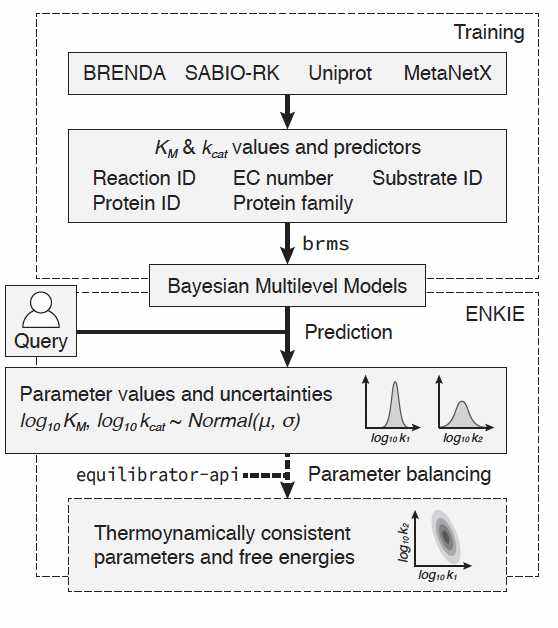
\includegraphics[width=0.5\linewidth]{1-enkie.png}
  \caption{ENKIE model overview}
  \label{fig:enkie}
\end{figure}

Published in Nature Communications, UniKP is a unified framework based on pretrained large language models
for predicting enzyme kinetic parameters: the enzyme turnover number ($k_{cat}$), the Michaelis constant
($K_m$), and the catalytic efficiency ($\frac{k_{cat}}{K_m}$). Similarly to \citeauthor{km1} is uses both the
protein sequence and the substrate string. It is comprised of 2 main components : a representation module 
for both the protein sequence (Figure \ref{fig:unikp}, part a) and the substrate string 
(Figure \ref{fig:unikp}, part b) and a machine learning module (Figure \ref{fig:unikp}, part c). 
Part d on Figure \ref{fig:unikp} are only relevent for $k_{cat}$ and include additional features into the model
such as pH and temperature. Part e of Figure \ref{fig:unikp} represents the re-weighting methods used 
to adjust the sample weight distribution to generate an optimized prediction. For the protein, the ProtT5-XL
model is used where, for each sequence, each amino acid is turned into a 1024-dimensional vector. To obtain
a condensed representation for each protein, mean pooling is applied. For the substrate, it is processed in
a similar way where each character of the string is processed by the SMILES-Transformer, resulting in a 
256-dimensional vector for each symbol. To get an equivalent 1024-dimensional vector for the substrate,
mean and max pooling are applied to these vectors and concatenated with the first and last output of the
model, as they are the start (SOS) and end of sequence (EOS). Then, both the protein and substrate representations
are contatenated and fed into the machine learning module. The latter is Extremely Randomized Trees, an
ensemble method that combines the predictions of multiple de-correlated decision trees to make more 
accurate and stable predictions than any single decision tree. It is similar to Random Forests but 
introduces extra randomness in the way splits are made at the nodes of the decision trees. \cite{extratrees}

\begin{figure}
  \centering
  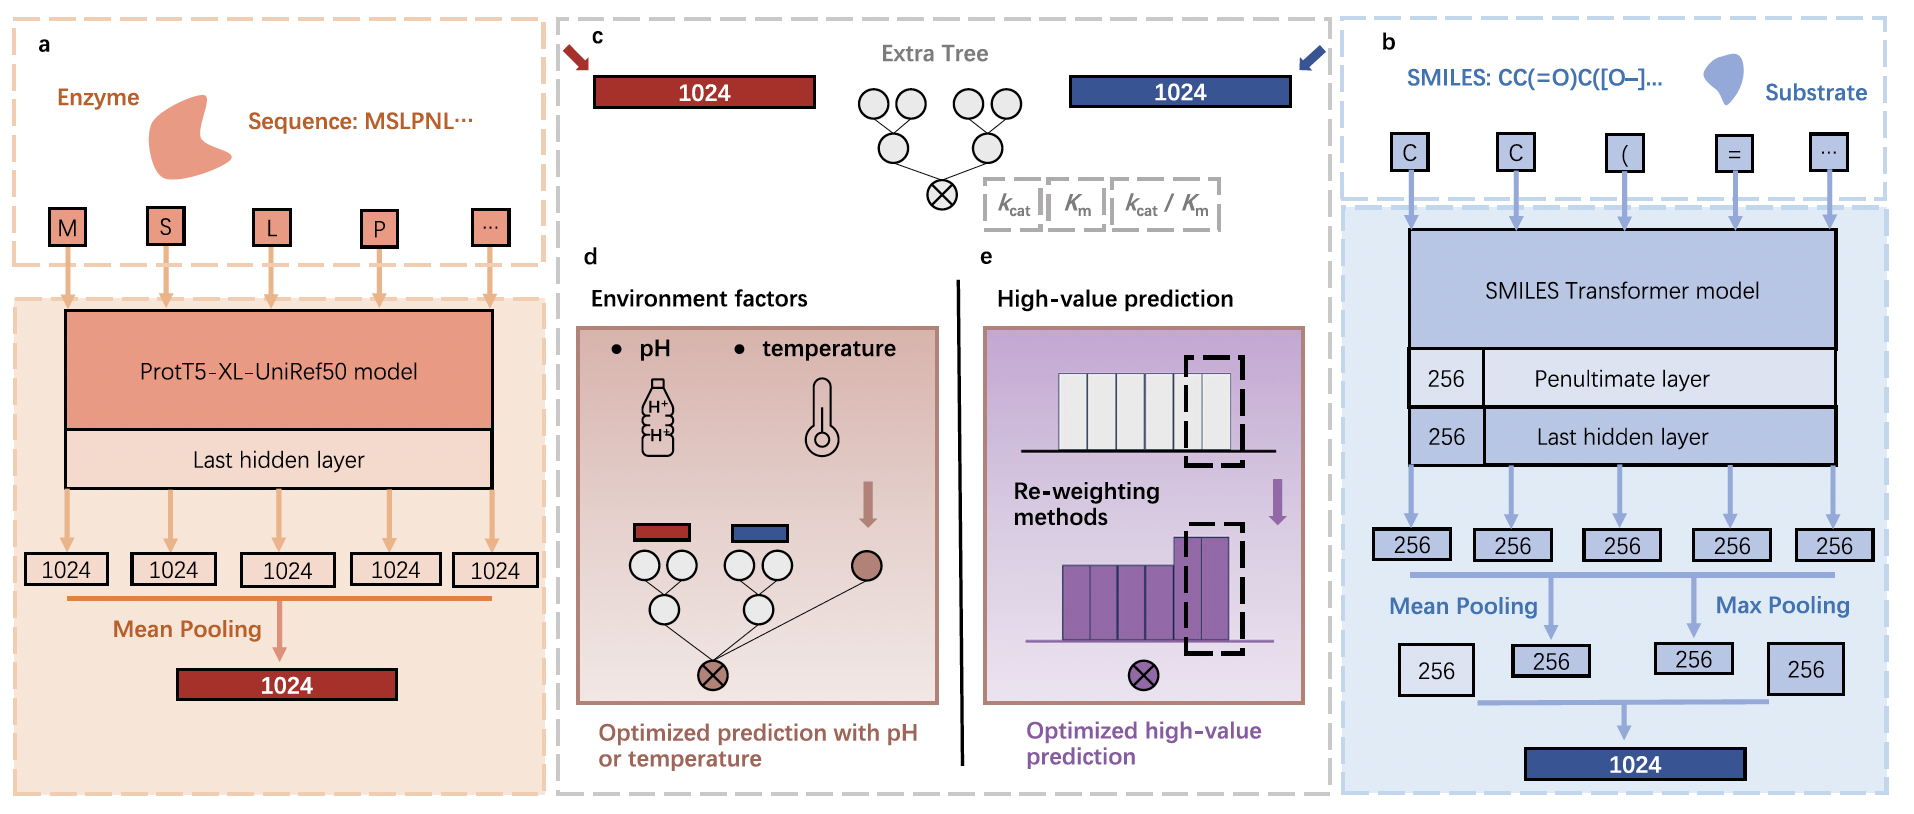
\includegraphics[width=1\linewidth]{1-unikp.png}
  \caption{UniKP model overview}
  \label{fig:unikp}
\end{figure}

Finally, the last method we will present is ProSmith. \cite{prosmith} While it hasn't been published yet
and is only available in preprint, it offers the best results for this task. This model employs a multimodal
transformer network to simultaneously process protein amino acid sequences and substrate strings. To do so,
the model use a concatenation approach where the protein sequence and substrate string are concatenated 
and separated by a separation token. In order to process this input, the network divide it into chunk 
known as tokens. For protein sequences, the tokens are the amino acids and for substrate, each symbol is
treated as a separate token. ProSmith use pre-learned token representations that were trained independently
on each modality. For amino acid representations, ESM-1b model was used and for the SMILES string tokens, it
was ChemBERTa2. \cite{esm1,chemberta} The token embeddings from ESM-1b and ChemBERTa2 have different dimensions,
1280 and 600 respectively. To process them using the same transformer network, the authors used linear layers
to map both sets of embeddings to a joint embedding space with a dimension of 768, which is also the hidden
dimension of all tokens in the ProSmith transformer network. 

\begin{figure}
  \centering
  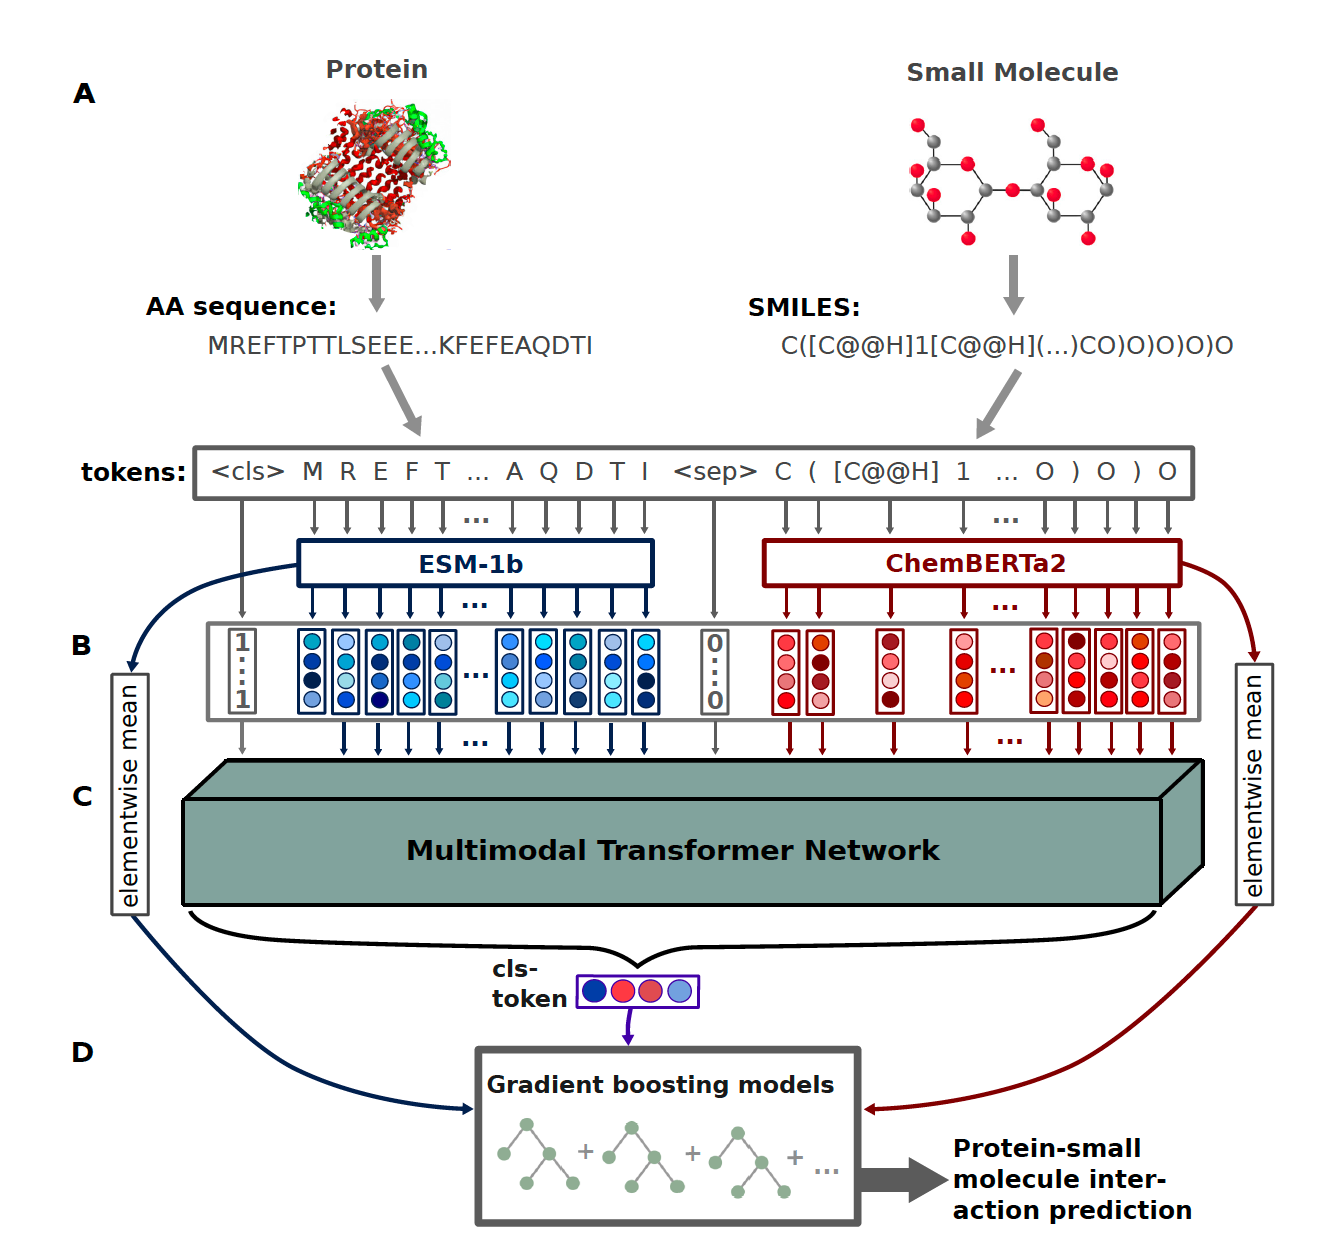
\includegraphics[width=1\linewidth]{1-prosmith.png}
  \caption{ProSmith model overview}
  \label{fig:prosmith}
\end{figure}

During the processing steps, the transformer 
network updates each input token using the attention mechanism, with 6 attention layers, each having
6 attention heads. \cite{attention} This enables the model
to look at the entire input sequence and selectly focus only on relevant token for making updates. 
After the update of all input tokens for a predefined number of steps, the classification token cls is
extracted and used as the input for a fully connected neural network, which is trained to predict an
interaction between the enzyme and the substrate. Then, the cls token, along with the original protein 
embedding from ESM-1b and substrate embedding from ChemBERTa2 are used as input to a gradient boosting model.
\cite{xgboost} This transformer model was pretrained on the Ligand-Target-Affinity Dataset from BindingDB.
\cite{bindingdb} All drug-target pairs with experimentally measured IC50 values were extracted and pairs 
that would be used for evaluation were removed. This results in 1,039,565 entries for the dataset. 95\%
were used for training ang 5\% for validation. The transformer network was trained for 100 epochs and saved
after each one. The model with the best results on the validation set was selected. Finally, the model
was fine-tuned for different tasks including the Michaelis constant on the dataset we discussed in this 
chapter.

The models presented have the following results:

\begin{table}[ht]
  \centering
  \begin{tabular}{lcc}
    \hline
    \textbf{Method} & \textbf{MSE \(\downarrow\)} & \textbf{\(R^2\) \(\uparrow\)} \\
    \hline
    ENKIE (2022) & -- & 0.463 \\
    Kroll et al. (2021) & 0.653 & 0.527 \\
    UniKP (2023) & 0.640 & 0.530 \\
    ProSmith (2023) & 0.604 & 0.563 \\
    \hline
  \end{tabular}
  \caption{Comparison of model performance for $K_m$ prediction}
  \label{tab:model_performance}
\end{table}


\section{Methodology}
This research will be composed of a data preprocessing step, a model implementation step, and an
evaluation step. Python 3.9 and PyTorch 2.0.1 will be used for these steps.

\subsection{Data preprocessing}
In this work, we will use the dataset prepared by \citeauthor{km1} and presented in the section \ref{sec:dataset}
The data used is up to 2022. Therefore, we will augment their dataset with a new test set composed of
the data from 2022 to January 2024, allowing a better testing of the current methods and the validation
of this work.
For all our model, we will therefore compute the metrics on the test set provided by the original dataset,
as well as on our new test dataset.
The processing of the new test set will be the same as for the original dataset.

\subsection{Model implementation}
The model implementation will be composed of 3 parts. The first one will be the creation of an architecture
for the sequence-based model, the for the structure-based model, and finally for the ensemble model using both
the sequence-based and the structure-based model.

\subsection{Model evaluation}
The 3 models of this work (sequence-based model, structure-based model, and sequence-structure-based model)
will be evaluated on the ProSmith test set as well as our newly curated test set. The evaluation metrics 
wil be the mean squared error (MSE) and the coefficient of determination $r^2$.

Not only will this work evaluate these metrics in the general sense but it will also provide a more specific
set of these metrics based on the data: the protein sequences and the substrates strings will be divided into
4 groups based on their appearance in the training set. Proteins that have been seen in the training set
will be denoted "hot proteins" and the ones that are not in the training set "cold proteins". Similarly, 
subrates included in the training set will be denoted "hot substrates" and "cold substrates" if they
are not.

These 4 groups will allow a better comparison of this work method and the state-of-the-art methods.

